\documentclass[11pt]{article}

\usepackage[T1]{fontenc}
\usepackage[utf8]{inputenc}
\usepackage[margin=1in]{geometry}
\usepackage{helvet}
\renewcommand{\familydefault}{\sfdefault}
\usepackage{xcolor}
\usepackage{tikz}
\usepackage{enumitem}
\usepackage{microtype}
\usepackage[hidelinks]{hyperref}
\setlength{\parindent}{0pt}
\setlength{\parskip}{6pt}

% --- palette ---
\definecolor{ink}{HTML}{0E1726}     % near-black brand ink
\definecolor{accent}{HTML}{49A078}  % Daytona-ish green accent
\definecolor{tierA}{HTML}{1F3A4D}   % model
\definecolor{tierB}{HTML}{2C6E7F}   % mcp
\definecolor{tierC}{HTML}{49A078}   % skills
\definecolor{cherry}{HTML}{E8553A}  % agent

\hypersetup{colorlinks=true, urlcolor=accent, linkcolor=accent}

\newcommand{\cake}{%
\begin{center}
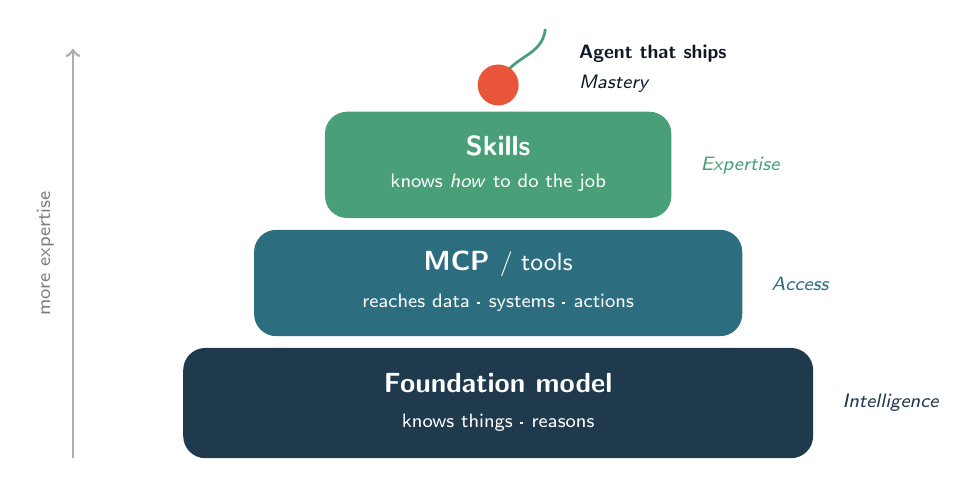
\begin{tikzpicture}[font=\sffamily, line width=0.6pt]
  % upward "expertise" arrow
  \draw[->, color=ink!35, line width=1pt] (-5.4,0) -- (-5.4,5.2);
  \node[rotate=90, color=ink!55, font=\scriptsize] at (-5.75,2.6) {more expertise};

  % Tier 1 — foundation model
  \fill[tierA, rounded corners=8pt] (-4,0) rectangle (4,1.4);
  \node[white] at (0,0.95) {\bfseries Foundation model};
  \node[white!85, font=\scriptsize] at (0,0.45) {knows things \textperiodcentered\ reasons};
  \node[tierA, right=7pt, font=\scriptsize\itshape] at (4,0.7) {Intelligence};

  % Tier 2 — MCP / tools
  \fill[tierB, rounded corners=8pt] (-3.1,1.55) rectangle (3.1,2.9);
  \node[white] at (0,2.46) {\bfseries MCP \textnormal{\small / tools}};
  \node[white!90, font=\scriptsize] at (0,1.98) {reaches data \textperiodcentered\ systems \textperiodcentered\ actions};
  \node[tierB, right=7pt, font=\scriptsize\itshape] at (3.1,2.22) {Access};

  % Tier 3 — Skills
  \fill[tierC, rounded corners=8pt] (-2.2,3.05) rectangle (2.2,4.4);
  \node[white] at (0,3.96) {\bfseries Skills};
  \node[white!92, font=\scriptsize] at (0,3.5) {knows \emph{how} to do the job};
  \node[tierC, right=7pt, font=\scriptsize\itshape] at (2.2,3.72) {Expertise};

  % Cherry — the agent
  \draw[accent, line width=1pt] (0,4.78) .. controls (0.25,5.15) and (0.55,5.1) .. (0.6,5.45);
  \fill[cherry] (0,4.74) circle (0.26);
  \node[ink, right=10pt, align=left] at (0.55,4.95)
    {\scriptsize\bfseries Agent that ships\\[-1pt]\scriptsize\itshape Mastery};
\end{tikzpicture}\\[2pt]
{\footnotesize\color{ink!60} The cake of agentic capability. Each tier adds a level of expertise --- and MCP and Skills are \emph{different tiers}, not competitors.}
\end{center}
}

\begin{document}
\thispagestyle{empty}

{\color{accent}\small\bfseries DAYTONA \ \textperiodcentered\ \ DOTFILES}\\[4pt]
{\fontsize{30}{34}\selectfont\bfseries\color{ink} Skills vs MCPs}\\[6pt]
{\large\color{ink!75} Two layers, one goal: agents that ship.}\\[2pt]
{\footnotesize\color{ink!55} 3 min read}

\vspace{4pt}
{\color{accent}\rule{\linewidth}{1.4pt}}
\vspace{6pt}

An MCP server hands an agent a box of tools. A Skill teaches it the craft to use them. They are not rivals --- they are different layers of the same cake. Today we are adding a new layer to Daytona: the \textbf{Daytona Skill} for Claude.

\textbf{\color{ink}Different layers, not competitors.}

\textbf{MCP is access.} It is the standardized wiring that lets an agent reach an external system. The Daytona MCP gives Claude twelve tools --- create a Sandbox, run a command, clone a repo, hand back a preview link.

\textbf{Skills are expertise.} A Skill is procedural know-how, loaded only when it is needed. The Daytona Skill teaches Claude \emph{when} to spin up a Sandbox, how to chain a build, when to snapshot, and to always clean up afterward.

The tell: tools tell an agent what it \emph{can} do. A Skill tells it \emph{how} to do the job well. You want both.

\cake

\textbf{\color{ink}The Daytona Skill.}

It packages everything we have learned about driving secure, sub-90-millisecond Sandboxes into a single playbook Claude reads on demand --- about 100 tokens of context until the moment it is needed, instead of a dozen tool definitions sitting in every conversation. And it drives the full Daytona SDK: persistent sessions, snapshots, volumes, and code execution --- the superset of what the MCP exposes.

MCP gives your agent reach. Skills give it judgment. Together they give it mastery --- agents that don't just write code, they ship it.

\vspace{4pt}
{\color{accent}\rule{\linewidth}{0.8pt}}
\vspace{2pt}

\textbf{The Daytona Skill is live.} \quad \href{https://www.daytona.io/docs}{Documentation} \ \textperiodcentered\ \ \href{https://github.com/daytonaio}{GitHub} \ \textperiodcentered\ \ \href{https://app.daytona.io}{Sign up}

\end{document}
